
\chapter{Gamma-ray Astrophysics}
\chaplabel{gamma_ray_astro}


\section{The History of Gamma-ray Astrophysics}
\seclabel{history_gamma_ray_detectors}

% Thorough discussion of all experiments:
%   http://imagine.gsfc.nasa.gov/docs/sats_n_data/gamma_missions.html
%   http://space.about.com/od/telescopesandoptics/a/Gammaray-Astronomy.htm

% Nice history with lots of pictures:
%  http://fermi.gsfc.nasa.gov/science/mtgs/symposia/2012/program/mon/DKniffen.pdf

% Good books with introduction

%  "Very High Energy Gamma Ray Astronomy" by Trevor C. Weekes
%    * seems to have a discussion of the principles of Gamma-ray detection.
%      scintilation detectors, spark chambers.

%  "Cosmic Gamma-Ray Sources" - edited by K.S. Cheng, Gustavo E. Romero

% Very nice reference:
%   http://adsabs.harvard.edu/abs/1984BASI...12..202P

% Nice summary:
%   http://articles.adsabs.harvard.edu/cgi-bin/nph-iarticle_query?1984BASI...12..202P&amp;data_type=PDF_HIGH&amp;whole_paper=YES&amp;type=PRINTER&amp;filetype=.pdf

Astronomy has historically been almost entirely concerned with studying
the photons that arrive from outer space.  Because of their charge
neutrality, photons are not defected by intergalactic electric and
magnetic fields and therefore point back to the objects 
emitting them. Historically, the field of astronomy concerned
the study of visible light.  Slowly, over time, astronomers 
expanded their view across the electromagnetic spectrum.

Infrared radiation from the sun was first observed by
William Herschel in 1980 \citep{herschel_1800_experiments-refrangibility}.
The first extraterrestrial source of radio waves was detected
by Jansky in 1933 \citep{jansky_1933_electrical-disturbances}.

% x-ray: http://en.wikiversity.org/wiki/Radiation_history#cite_ref-Burnight_183-1
The development of rockets and sattelites in the 20th ceuntry allowed
the field of astronomy to expand futher, allowering observations
at wavelengths that would otherwise be absorbed in the atmosphere.
The first ultraviolet observation of the sun was performed in 1946 from a
captured V-2 rocket \citep{baum_1946_ultraviolet-spectrum}.  Observations of
solar x-rays were also first carried out on a captured V-2 Rocket in
1949 \citep{burnight_1949_x-radiation-atmosphere}

It was only natural to wonder about the universe at even higher energies.
As is common in the field of physics, the prediction of
the detection of cosmic $\gamma$-rays far proceded their discovery.
\cite{feenberg_1948_interaction-cosmic-ray} theorized that the interaction
of starlight with cosmic rays could produce $\gamma$-rays through
\ac{IC} upscattering.  Following the discovery of the neutral
pion in 1949, \cite{hayakawa_1952_propagation-cosmic}
predicted that $\gamma$-ray emission could be observed from the
decay of neutral pions when cosmic rays interacted with interstellar
matter.  And in the same year, \cite{hutchinson_1952_possible-relation}
discussed the bremsstrahlung radiation of cosmic-ray electrons.
\cite{morrison_1958_gamma-ray-astronomy} first predicted the detection
of several sources of $\gamma$-rays including solar flares, \acp{PWN},
and active galaxies.

\todo[inline]{
Why Gamma-rays can't make it to the ground
}
    
\todo[inline]{Discuss
Balloon gamma-ray detectors.
See discussion on p859 (comparison with other 
experiments) of Kraushaar et al 1965. 
What was the background from, earth albedo gammas I think?
See also Kraushaar et al 1972 p342's discussion of the balloon
experiments: Hulsizer and Rossi (1949), ... 
See also William Tomkin's section 2.2.1 on 
Balloon experiments (page 8) for references
to galactic plane emission being measured
by balloon experiments in 1970.}


    % Links on Explorer 11
% en.wikipedia.org/wiki/Explorer_11
%http://www.physics.wisc.edu/news/obits/kraushaar_obit.html
% http://heasarc.nasa.gov/docs/heasarc/missions/explorer11.html#reference
% http://articles.adsabs.harvard.edu/cgi-bin/nph-iarticle_query?1965ApJ...141..845K&amp;data_type=PDF_HIGH&amp;whole_paper=YES&amp;type=PRINTER&amp;filetype=.pdf

% "The instrument package weighed 30 pounds, was 20 inches high and 10 inches in diameter. The experimenters believed that they detected 22 cosmic gamma rays."
%  -> http://imagine.gsfc.nasa.gov/docs/sats_n_data/gamma_missions.html
The first space-based $\gamma$-ray detector was \explorerxi
\cite{kraushaar_1965_explorer-experiment}.  It was developed at \ac{MIT}
under the direction of William L. Kraushaar.  It employed a sandwich
scintillator and a Cherenkov counter to direct the position and energy
of incoming $\gamma$-rays and was surounded by a plastic anticoincidence
scintilation counter. The sandwich detector had an area of $\sim45\cm^2$,
but an effective area of only $\sim 7\cm^2$, corresonding
to a detector efficiency of $\sim 15\%$.

\todo[inline]{What was the energy range of explorer ii}

It was launched on boad \explorerxi on April 27,
1961. The instrument was in opreation for 7 months, but only 141 hours
of data were of acceptable quality.  Using these observations, \explorerxi
observed 31 $\gamma$-rays and, because the distribution a distribution of
these $\gamma$-rays was consistent with being isotropic, the experiment
could not firmly identify the $\gamma$-rays as being cosmic in nature.


% en.wikipedia.org/wiki/OSO_3
% "Their
% next detector, on Orbiting Solar Observatory -3, may be more accurately
% described as having proof of the discovery of cosmic gamma radiation,
% since it found a galactic plane anisotropy of high-energy gammas, much
% later to be confirmed with SAS-2 and COS-B." -- http://imagine.gsfc.nasa.gov/docs/sats_n_data/gamma_missions.html

% Notes: 621 photons, E>100 GeV, 1967, angular resolution +/- 16deg from 
%  ``Cosmic Gamma-Ray Sources`` K.S. Chen, Gustavo E. Romer

\todo[inline]{Describe scintilation detector better.
Read William Tomkin's thesis, page 8.}

The first definitive detection of $\gamma$-ray came in
1962 by an experiment on the Ranger 3 moon
probe \citep{arnold_1962_gamma-space}.  It detected an isotropic flux
of $\gamma$-rays in the 0.5 \mev to 2.1 \mev energy range.

\ac{OSO-3}, also developed by Kraushaar, followed \explorerxi
as the next major astrophysical $\gamma$-ray detector
\cite{kraushaar_1972_high-energy-cosmic}.  The \ac{OSO-3} sattelite
allowed the on board $\gamma$-ray detected to have an improved weight,
power, telemetry, and expsoure, creating a more sensitive experiment.
The experiment operated in the energy range from 50 \mev to $\sim 400$
\mev and had an effective area $\sim 9$ $\cm^2$.

It was launched on March 8, 1967 and operated for 16 months, measuring
621 cosmic $\gamma$-rays.  The most important result of the expirment was
to measure a strong anisotrophy in the distribution of the $\gamma$-rays
with a strong clustering of $\gamma$-rays towards the Galactic plane.
\figref{oso3_skymap} shows a skymap of these $\gamma$-rays.  This
experiment confirmed both a Galactic component to the $\gamma$-ray
sky as well as an additional isotropic component, hypothesised to be
extragalactic in origin.

\todo[inline]{What was the PSF of OSO-3? could it be pointed?}

\begin{figure}[htb]
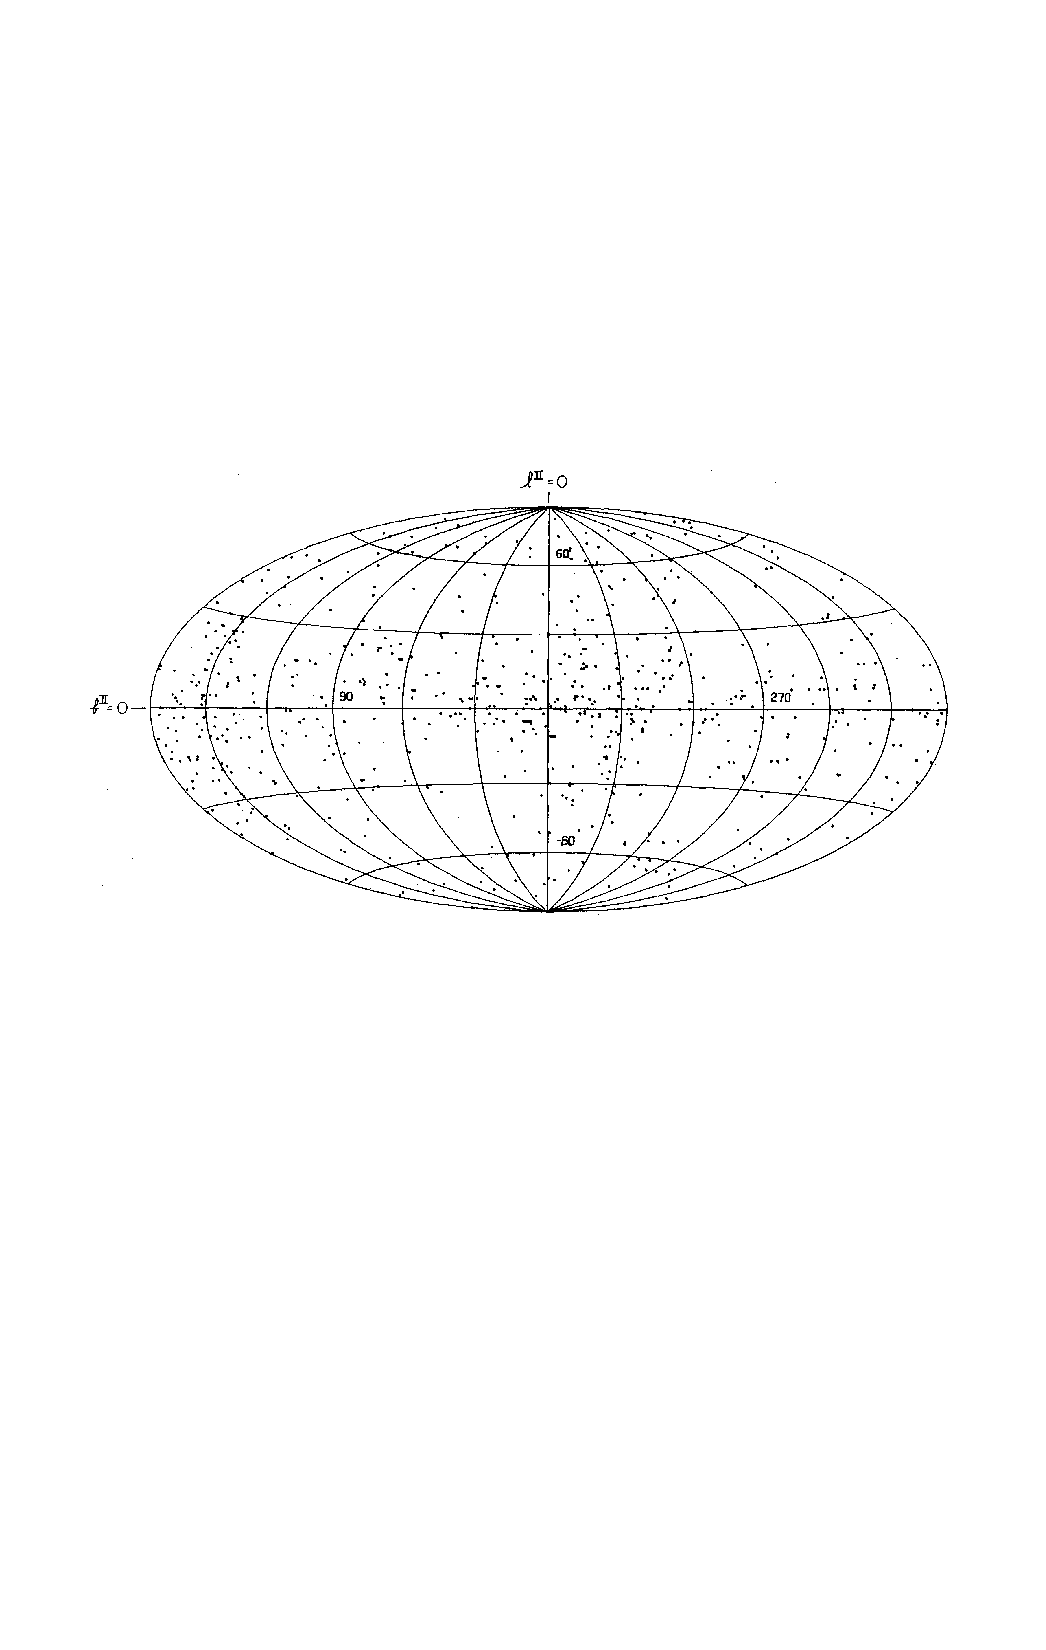
\includegraphics{chapters/introduction/figures/kraushaar_et_al_1972_skymap.pdf}
\figlabel{oso3_skymap}
\caption{The position of all 621 cosmic $\gamma$-rays
detected by \ac{OSO-3}. This figure is from 
\cite{kraushaar_1972_high-energy-cosmic}. }
\end{figure}

% ``The field of gamma-ray astronomy took great leaps forward'' -- wikipedia

  % ``Additional gamma-ray experiments flew on the OGO, OSO, Vela, and Russian
  % Cosmos series of satellites. However, the first satellite designed as a
  % ``dedicated'' gamma-ray mission was the second Small Astronomy Satellite
  % (SAS-2) in 1972.`` - http://imagine.gsfc.nasa.gov/docs/science/know_l1/history_gamma.html



The next major advancement in $\gamma$-ray astronomy came from
the \ac{SAS-2} and \cosb missions.

\ac{SAS-2} was a dedicated $\gamma$-ray detector
launched by \ac{NASA} in November 15, 1972.  \ac{SAS-2} was
\cite{fichtel_1975_high-energy-gamma-ray} It improved upon \ac{OSO-3}
by incorporating a spark chamber and having an overall larger size.
The size of the active area of the detector was 640 $\cm^2$ and the
experiment had a much improved effective area of $\sim 115\,cm^2$. The
spark chamber allowed for a seperate measurement of the electron and
positron tracks, which allowd for improved directional reconstruction
of the incident $\gamma$-ray. \ac{SAS-2} had a PSF $\sim5\degree$ at 30
\mev and $\sim1\degree$ at 1 \gev.

\ac{SAS-2} collected data for over 6 months before a power supply
failure ended data collection. \ac{SAS-2} Observed over 8,000
$\gamma$-ray photons covering $\sim55\%$ of
the sky including most of the Galactic plane.  
\ac{SAS-2} disovered strong emission
along the Galactic plane and particularly towards the Galactic
cente. It also discovered
pulsations from the
Crab \citep{fichtel_1975_high-energy-gamma-ray} and Vela pulsar
\citep{thompson_1977_sas-2-high-energy}.  In addition, \ac{SAS-2}
discovered Geminga, the first $\gamma$-ray source with no compelling
multiwavelenth counterpart \citep{thompson_1977_final-sas-2}. Gemina
was eventually discovered to be a pulsar by \ac{EGRET}
\citep{bertsch_1992_pulsed-high-energy} and retroactivly by \ac{SAS-2}
\citep{mattox_1992_observation-pulsed}.

% ``Cos-B was ESA's first satellite dedicated to a single experiment. Its
% scientific mission was to study in detail the sources of extra-terrestrial
% gamma radiation at energies above about 30 MeV. The originally foreseen
% duration of the mission was two years, but in fact Cos-B functioned
% successfully for 6 years and 8 months. During this time an extensive
% survey of the Galaxy was made in the energy range 50 MeV to 5 GeV.''
% -- http://sci.esa.int/science-e/www/area/index.cfm?fareaid=34

% ``Description Cos-B was the first ESA mission dedicated to the study of
% gamma-ray sources. Its results created a catalogue of these sources,
% known as the 2CG Catalogue, the first complete map of the gamma-ray
% emission from the disc of our Galaxy, the Milky Way, and the first
% detectable emission from an extra-galactic object 3C273.'' 
% -- http://www.esa.int/Our_Activities/Space_Science/Cos-B_factsheet

% cos b performance is described at:
%   http://www.rssd.esa.int/index.php?page=gr-tele&project=COSB

\cosb, an \ac{ESA} mission, was launched shortly after, on August
9, 1975.  Similar to \ac{SAS-2}, \cosb includd a spark chamber for
reading out the $\gamma$-ray events and had a peak effective area
of $\sim 50\,cm^2$ at $\sim400\,MeV$ It improved upon the design
\ac{SAS-2} by including a calorimiter below the spark chamber which
improved the energy resolution to $<100\%$ for energies $\sim 3\,\gev$
\citep{bignami_1975_cos-b-experiment}.

\cosb operated successfully for over 6 years and produced
the first detailed catalog of the $\gamma$-ray sky.
\ac{2CG} detailed the detection 25 $gamma$-ray sources
for $E>100\,\mev$ \citep{swanenburg_1981_second-catalog}.

\begin{figure}[htb]
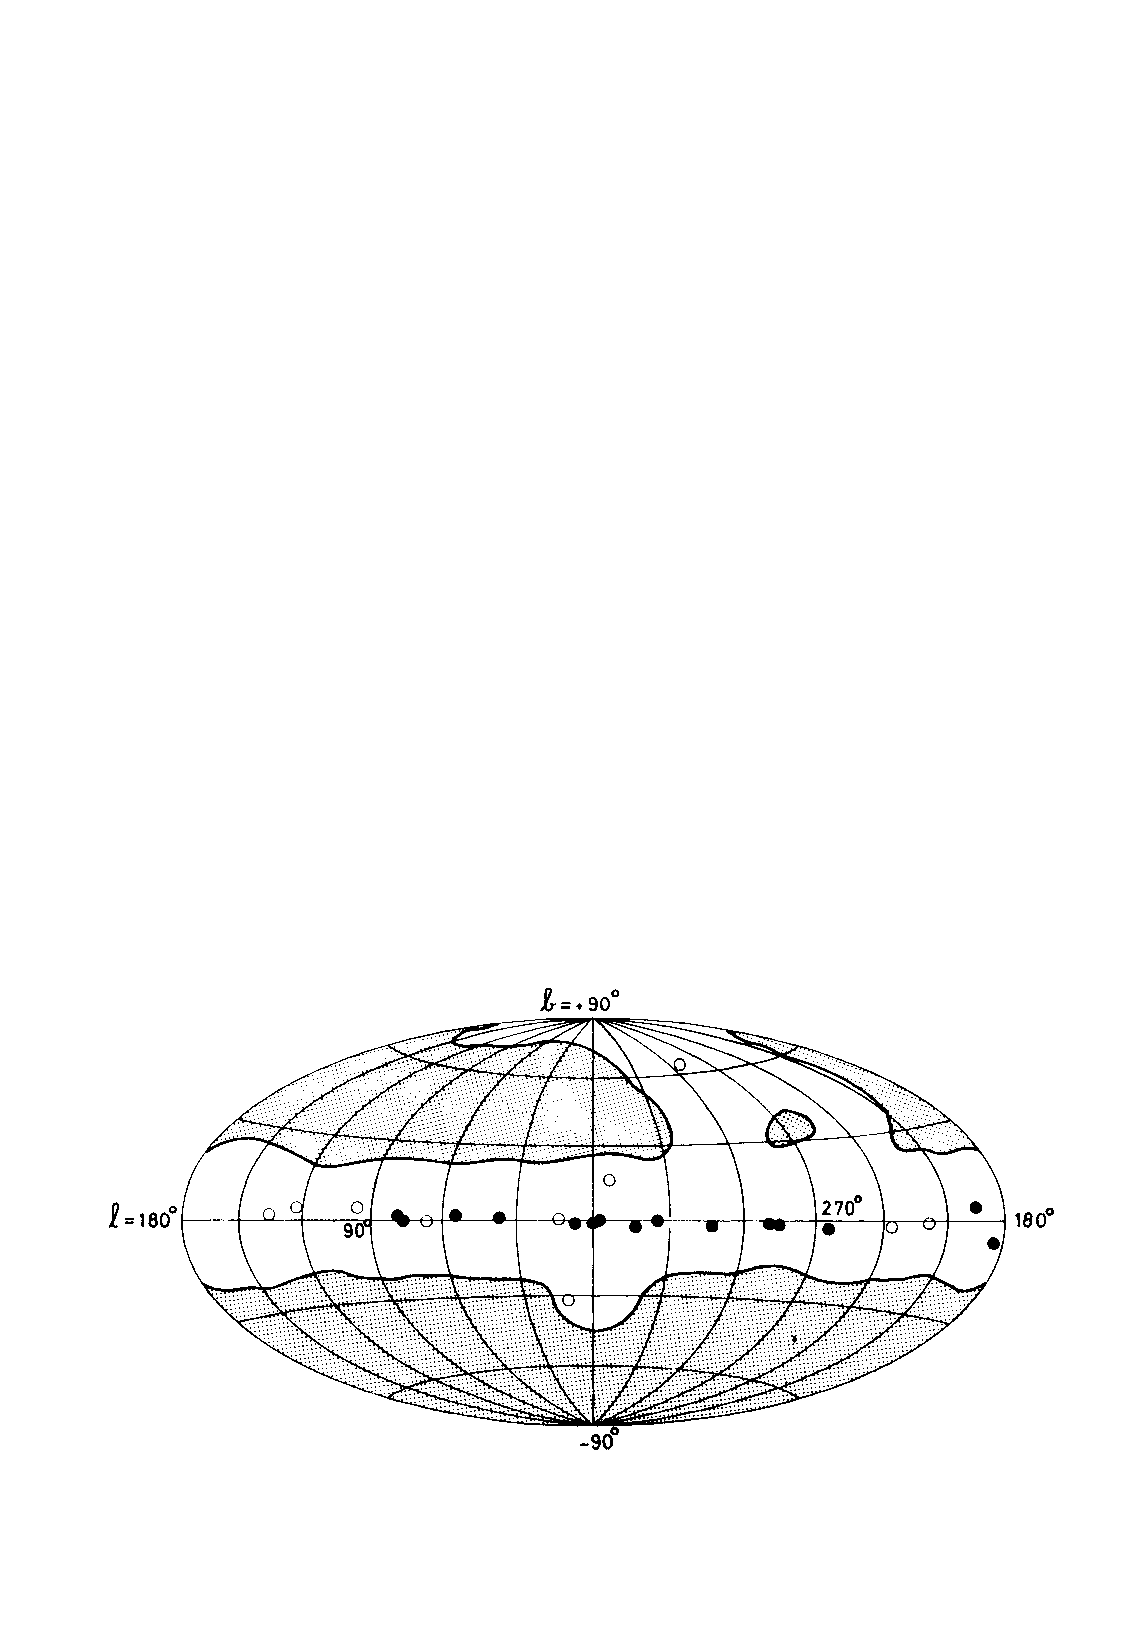
\includegraphics{chapters/introduction/figures/cos_b_2nd_catalog.pdf}
\figlabel{cos_b_skymap}
\caption{
The figure is from \cite{swanenburg_1981_second-catalog}.
}
\end{figure}


\todo[inline][3C27]

% 6 years and 8 months. During this time an extensive survey of the Galaxy was made in the energy range 50 MeV to 5 GeV.

: 2 Year catalog: 
\todo[inline]{Describe COS-B. What was its effective area}



\begin{itemize}
  \item EGRET
    % Good summary of EGRET Results:
    %  http://arxiv.org/pdf/0811.0738.pdf
  \item AGILE
  \item \todo[inline]{Short description of the history
    of TeV astronomy}
\end{itemize}





\section{Astrophysical Sources of Gamma-ray}

\subsection{Pulsar Wind Nebulae}

% Good history of observations of crab nebulae:
%  * chapter 1 of "The Crab Nebula" by Rodney Deane Davies

% good history paper: http://arxiv.org/pdf/1211.0852.pdf

\todo{First nebulae?}


\subsection{Pulsars}

% good details from "Pulsar Astronomy" By Andrew G. Lyne, Francis Graham-Smith

Pulsars were first discovered in 1967 by Jocelyn Bell Burnell and Antony
Hewish \citep{hewish_1968_observation-rapidly}. They had constructed a
radio telescope that used interplanetary scintillation wiht the intention
of observing quasars.  In the process, they detected a source with a
periodicity of 1.3 \second.

Even before the discovery, \cite{pacini_1967_energy-emission} had predicted
the existence of neutron stars.  Shortly following the 1967 discovery,
\cite{gold_1968_rotating-neutron} and \cite{pacini_1968_rotating-neutron}
argued that the observed pulsar was a rotating neutron star.

The discovery of many more pulsars came quickly.  In 1968, and the
Vela pulsar \citep{large_1968_pulsar-supernova} and the Crab pulsar
\citep{staelin_1968_pulsating-radio} were discovered.

% Info came from the book ``Pulsar Astronomy'' by Lyne.
The first pulsar observed at optical frequencies was the
Crab, discovered in 1969 shortly after its radio discvoery
\citep{cocke_1969_discovery-optical}.
In the same year, the first X-ray pulsations were discovered from
the same source. At the time, there were no space-based X-ray
observatories, so observations had to be performed from rockets.
The discovery was carried out almost concurrently by a group
at \ac{NRL} \citep{fritz_1969_x-ray-pulsar} and at \ac{MIT}
\citep{bradt_1969_x-ray-optical}.  Using proportional counters,
these experiments showed that the pulsed emission from 
the Crab extended to X-ray energies and that, for this source,
the X-rays emission was a factor $>100$ more energetic than
the observed visible emission.

As was discussed in \secref{history_gamma_ray_detectors},
$\gamma$-ray emission from the Crab was detected only 2 years
later \citep{browning_1971_detection-pulsed}.

\todo{First gamma-ray detection}

ATNF catalog?

EGRET pulsars?

The state of the art in $\gamma$-ray detection of pulsars
will be included in an upcomming pulbication.
2PC: \secref{second_pulsar_catalog}

\todo[inline]{When was the PSR, PWN connection made}

\todo[inline]{Describe pulsar physics. See description from Carroll and Ostlie page 593}
\begin{equation}
  \energydot = 
  -4\pi^2 \momentofinertia \perioddot/\period^3
\end{equation}

\begin{equation}
  \pulsarage = \period/2\perioddot
\end{equation}



\subsection{Supernova Remenants}



\section{The \fermi Gamma-ray Space Telescope}
\seclabel{fermi_telescope}

\begin{figure}[htbp]
  \centering
    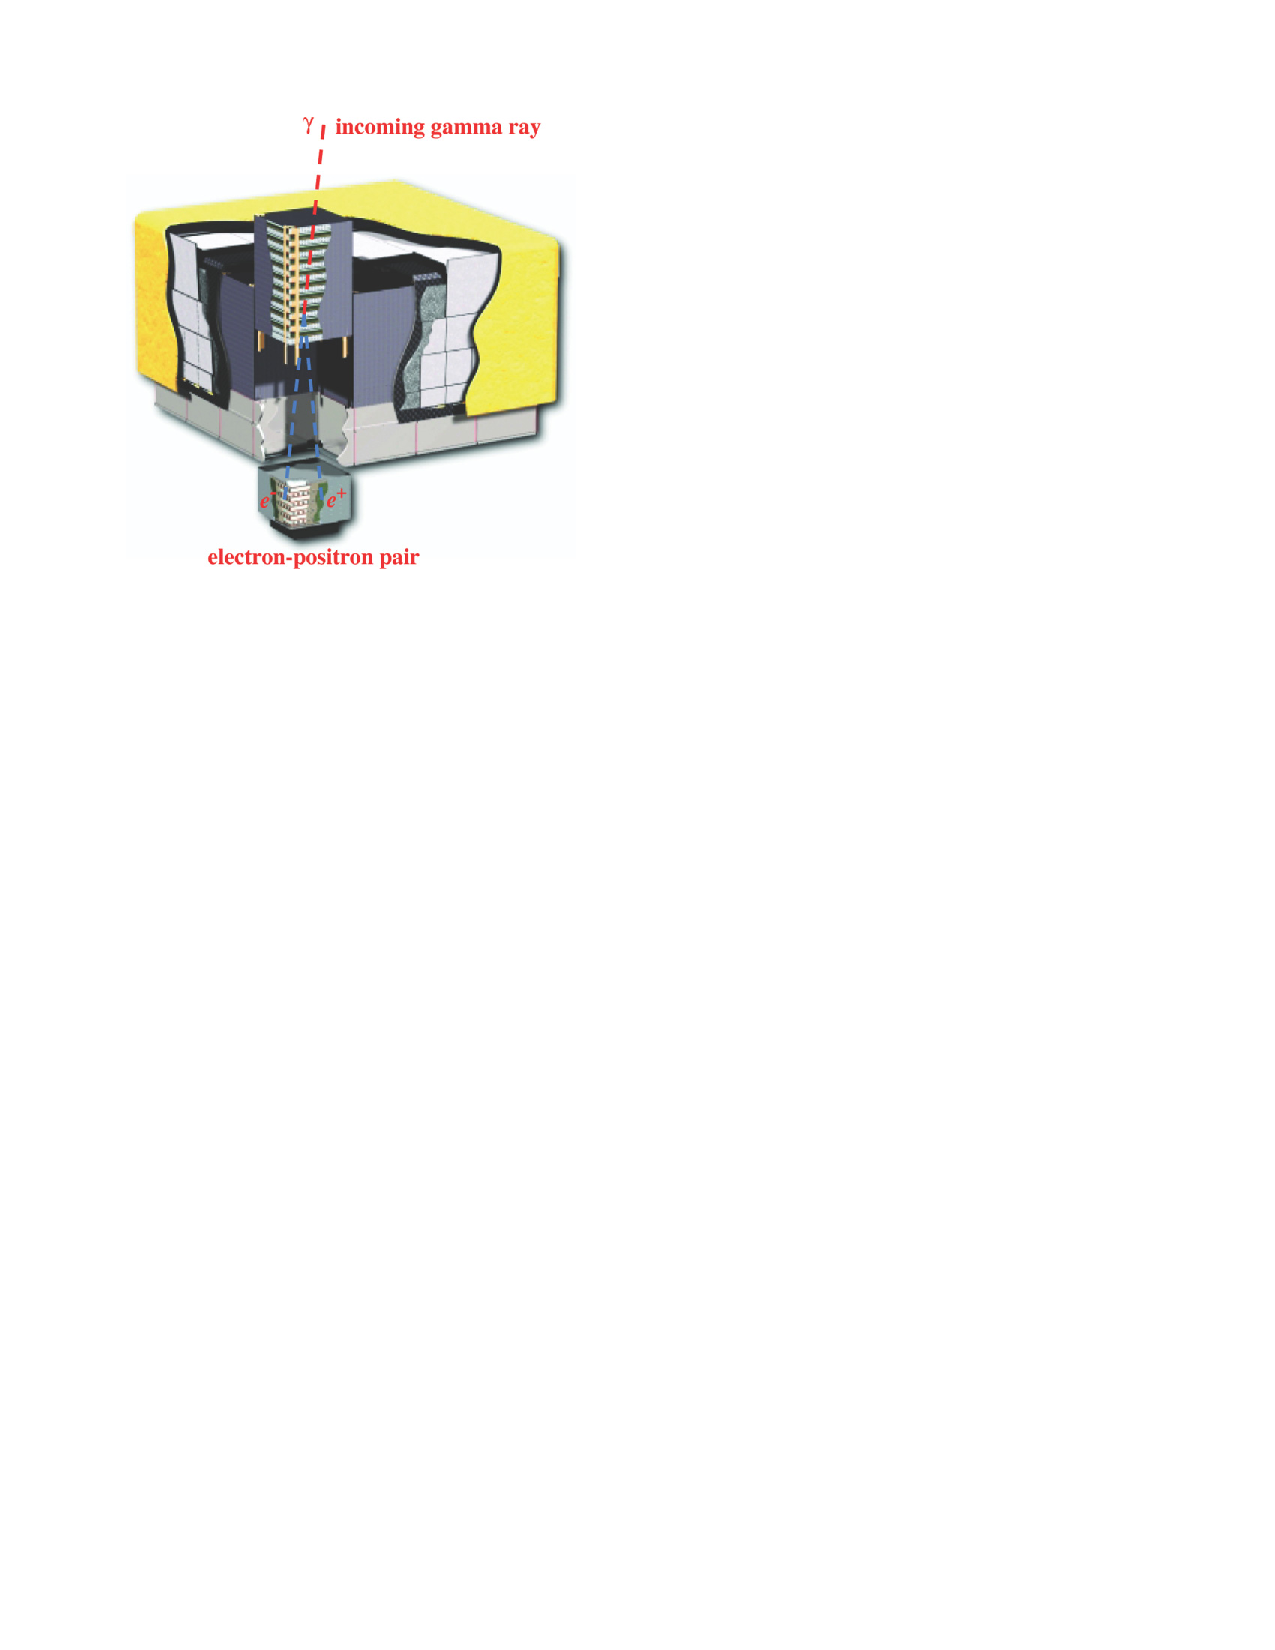
\includegraphics{chapters/introduction/figures/lat_detector_cutout.pdf}
  \caption{A schematic diagram of the \ac{LAT} with an incident $\gamma$-ray
    (red line) pair-converting into an electron and positron (blue lines)
    which are recorded in the tracker and calorimiter of the \ac{LAT}.
    This figure is taken from \citep{atwood_2009a_large-telescope}.  
    This diagram shows the three major subsystems of the \ac{LAT}:
    the tracker, the calorimiter, and the \ac{ACD}.
  }
  \figlabel{lat_detector_cutout}
\end{figure} 


The \fermi Gamma-ray Space telescope was launched on June 11, 2008 on
a Delta II heavy launch vehicle \citep{atwood_2009a_large-telescope}.
The primary since instrument on board \fermi is the \ac{LAT},
which is a pair-conversion telescope which detects $\gamma$-rays
in the energy range from $20\unitspace\mev$ to $>300\unitspace\gev$.
\figref{lat_detector_cutout} shows a schematic diagram of the \ac{LAT}.
With its unprecedent effective area and angular resolution, the \ac{LAT}
has drastically improved our understanding of the $\gamma$-ray sky.
In addition, \fermi contains the \Ac{GBM}, which is used to obseerve
\acp{GRB} in the energy range from $\sim8\unitspace\kev$ to $\sim40\unitspace\mev$.
See \cite{meegan_2009a_fermi-gamma-ray} for a description of the \ac{GBM}
detector.

\subsection{The \acs{LAT} Detector}

The \ac{LAT} is composed of three major subsystems: the tracker, the
calorimeter, and the \ac{ACD}. Fundamentally, the detector operates by
inducing an incident $\gamma$-ray to pair convert in the tracker into
an electron and positron pair. The electron and position travel through
the tracker and into the \ac{CsI} calorimiter.  The track they leave in
the tracker and the energy deposite they leave in the calorimter can be
used to infer the direction and energy of the incident $\gamma$-ray.

Both the tracker and calorimiter are $4\times4$ arrays, each composed of
16 modules.  Each tracker tower is divided into 18 tungsten converter
layers and 16 dual-silicon tracker planes ($x$ and $y$).  As a balance
between effective area and angular resolution, The top 12 tracker planes
have thin layers of tungsten which minimize the probability of secondary
scattering and improves the angular resolution of the \ac{LAT}, especially
for low-energy $\gamma$-rays. The bottom four tracker planes have layers
of tungsten $\sim6$ times thicker, which improves the likelihood of
conversion and therefore the effective area.  The ``front'' and ``back''
classificaiton for $\gamma$-rays refers to if they convert in the thin
or thick layers of the detector, respectivly.  Each calorimiter module
composed of eight layers of 12 \ac{CsI} crystals. The depth of the
calorimiter is 8.6 radiation lenghts adn the depth of entire insutrment
is 10.1 radiation lenths.

The \ac{ACD}, the third subsystem on the \ac{LAT}, provides provides
background rejection by of the charged particle background incident
on the \ac{LAT}.  The \ac{ACD} surrounds the tracker and is composed
of 89 plastic scintillator tiles ($5\times5$ on the top and 16
on each of the sides). The \ac{ACD} has a 0.9997 efficiency for
detcting singly-charged particles entering the \ac{LAT}.  A detailed
discussion of the various subsystems of the LAT can be found in
\citep{atwood_2009a_large-telescope}.

\subsection{Performance of the \acs{LAT}}

The \ac{LAT} 
has an unprecidended effective area ($\sim9,500\unitspace\cm^2$),
single-photon energy resolution ($\sim10\%$), and single-photon
angular resolution ($\sim3\fdg5$ at $\energy=100\unitspace\mev$
and decreasing to $\lesssim0\fdg15$ for $\energy>10\unitspace\gev$)
\citep{atwood_2009a_large-telescope}.

With its $2.4\unitspace\steradian$ filed of view,

\todo[inline]{forward reference description of analysis of LAT data}


\section{Radiation Processes in Gamma-ray Astrophysics}

Nontermal radiation observed from astrophysical sources
is typically believed to originate in syncrotron
\ac{IC}, and the decay of neutral \pion particles.

\subsection{Synchrotron}


\begin{figure}[htbp]
  \centering 
    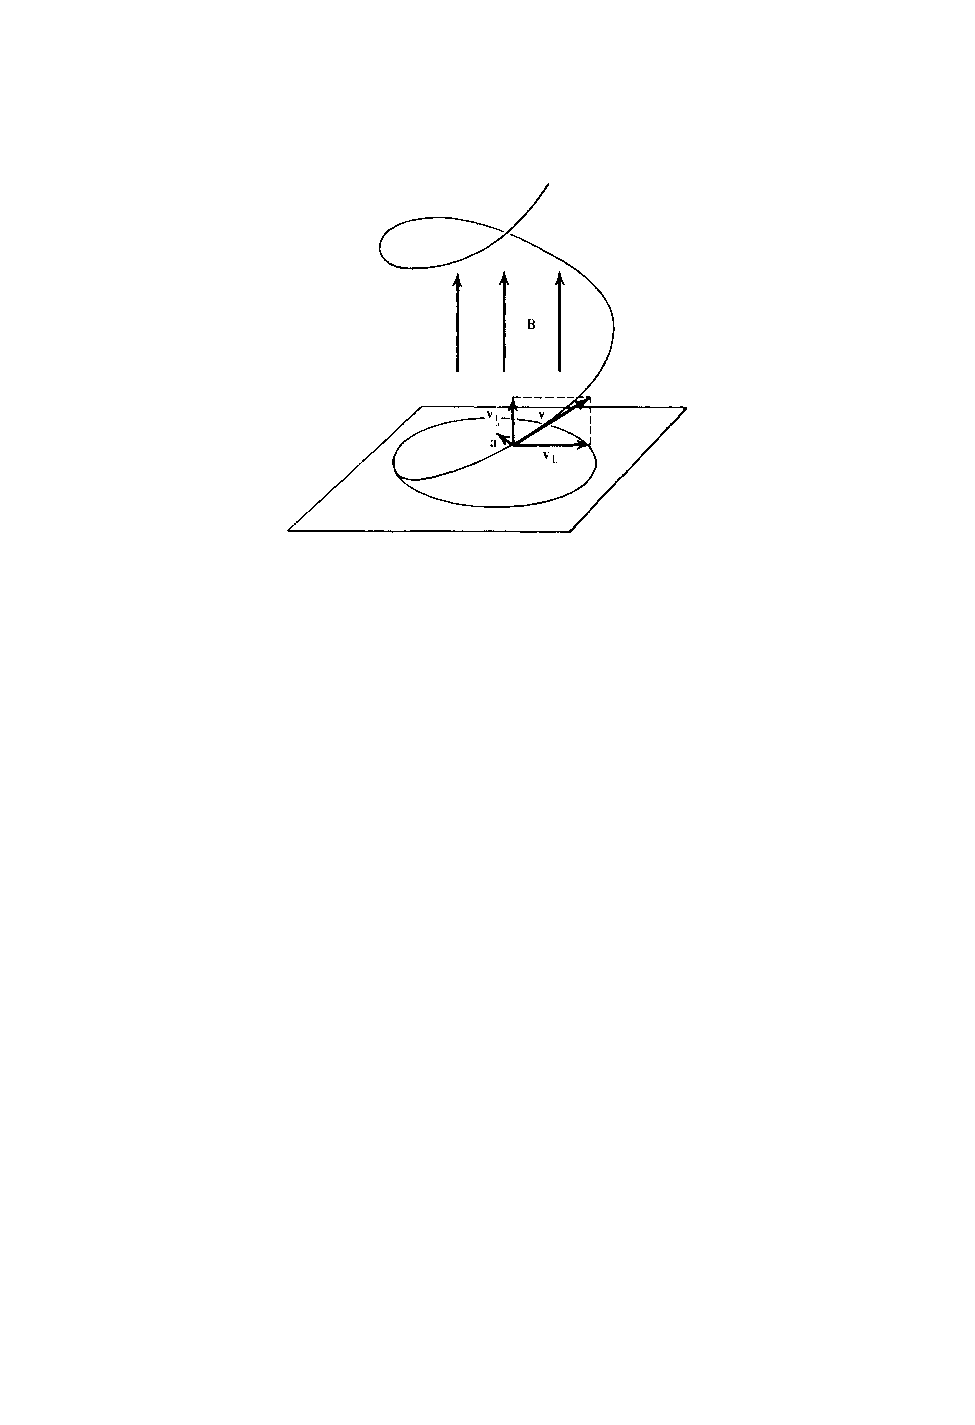
\includegraphics{chapters/introduction/figures/syncrotron_radiation_spiral.pdf}
    \caption{In synchrotron radiation, charged particles spiral along
      magnetic filed lines, radiating photons as they accelerate.}
  \figlabel{syncrotron_radiation_spiral}
\end{figure}


The synchrotron radiation processes is commonly observed in
astrophysics. It is caused when charged particles, typically
electrons, spiral around magnetic field lines.  As they
accelerate, they radiate photons.  This process is illustrated in
\figref{syncrotron_radiation_spiral}.
This emission is discussed thoroughly in
\cite{blumenthal_1970a_bremsstrahlung-synchrotron} and
\cite{rybicki_1979a_radiative-processes}.
In what follows, we adopt the notation from
\cite{houck_2006a_models-nonthermal}.

A charged particle of 
mass $\mass$ and charge $\charge$ in a magnetic field
of strength 
\MagneticFieldVector
will experince an
electromagnetic force:
\begin{align}
% equation 6.1a in R&L 1979
  \dbydt (\gamma m \VelocityVector) = & \frac{q}{c} \cross{\VelocityVector}{\MagneticFieldVector}
\end{align}
This force will cause a particle to accelerate around
the magnetic field lines, causing it
to radiate by maxwell's equations.

The power emitted at a frequency $\frequency$ 
by particle spiraling will be
\begin{equation}
% equation 6.33 in R&L 1979
  \eqnlabel{power_emitted_particle_sync}
  \power_\text{emitted}(\frequency) = 
  \frac{\sqrt{3} \charge^3 B \sin\alpha}{\mass \speedoflight^2} F(\frequency/\frequency_c)
\end{equation}
where $\alpha$ is the angle between the particle's velocity vector and
magnetic field vector.
Here,
% equation 6.31c in R&L 1979
\begin{equation}
  F(x) \equiv x \int_x^\infty K_{\tfrac{5}{3}} (\xi) d\xi,
\end{equation}
and
\begin{equation}
% equation 6.11a in R&L 1979
\frequency_c = \frac{3q \MagneticField \gamma^2}{4\pi \mass \speedoflight} 
\sin\alpha \equiv \nu_0 \gamma^2 \sin\alpha
\end{equation}

Because power is inversely-proportional to mass, synchotron radiation
is almost always assumed to come from electrons.

Now, we assume a population of particles and compute the total
emission. We say that $\ParticleDistribution(\momentum,\alpha)$ is the number of particles
per unit momentum and solid angle with a momentum $\momentum$ and
pitch angle $\alpha$.

We find the total power emitted by integrating over particle
momentum and distribution
\begin{equation}
  \frac{\derivative W}{\derivative\time}=
  \int \derivative \momentum 
  \int \derivative \solidangle
  \power_\text{emitted}(\frequency)
  \ParticleDistribution(\momentum,\alpha)
\end{equation}
If we assume the pitch angles of the particles to be isotropically
distributed and include \eqnref{power_emitted_particle_sync}, we
find that the photon emission per unit energy and time is
\begin{equation}
  \frac{\derivative \ParticleDistribution}{\derivative \omega \derivative \time} =
  \frac{\sqrt{3}q^3 B}{h m_e c^2 \angularfrequency}
  \int \derivative\momentum
  \ParticleDistribution(\momentum)
  R \left(\frac{\omega}{\omega_0 \gamma^2}\right)
\end{equation}
where
\begin{equation}
  R(x) \equiv \frac{1}{2} \int_0^\pi
  \derivative \alpha \sin^2 \alpha
  F\left(\frac{x}{\sin\alpha}\right)
\end{equation}

It is typical in astrophysics to assume a 
a power-law distribution of electrons written as
\begin{equation}
% equation 6.20a in R&L 1979
\eqnlabel{ElectronPowerLawEnergyDistribution}
  \ParticleDistribution(\momentum) \derivative\momentum = 
  \kappa \momentum^{-\spectralindex} \derivative\momentum.
\end{equation}
For a powerlaw distribution of photons integrated over
pitch angle, we find
\begin{equation}
\TotalPower(\angularfrequency) \propto \kappa \MagneticField^{(p+1)/2} 
\angularfrequency^{-(p-1)/2}.
\end{equation}
See, \cite{rybicki_1979a_radiative-processes} 
or \cite{longair_2013a_energy-astrophysics} for a full derivation.
This shows that, assuming a power-law electron distribution,
the electron spectral index can be related to the photon spectral
index.

\subsection{\Actitle{IC}}

Normal compoton scattering involves a photon colliding with a free electron
and transfering energy to it. In \ac{IC} scattering, a high-energy 
electron interacts with a low-energy photon imparting energy to it.
This process occurs when highly-energetic electrons interact with
a dense photon field.

The derivation of \Ac{IC} emission requires a quantum
electrodynamical treatment. It was first computed in
\cite{klein_1929a_streuung-strahlung}, and the derivation is described
in \cite{blumenthal_1970a_bremsstrahlung-synchrotron}.  In what follows, we follow
the notational convetion of \cite{houck_2006a_models-nonthermal}.

We assume a population of relativistic ($\gamma\gg1$) electrons
written as $\ParticleDistribution(\momentum)$ which is contained inside isotropic 
photon distribution with number density $n(\omega_i)$.

The distribution of photons 
emitted by \ac{IC} scatter is
written as
\begin{equation}
  \frac{\derivative\ParticleDistribution}{\derivative\omega\derivative\time} = 
  c \int d \omega_i n(\omega_i)
  \int_{p_\text{min}}^\infty  dp
  \ParticleDistribution(p) 
 \KleinNishinaCrossSection(\gamma,\omega_i,\omega)
\end{equation}
where $\omega$ is the outgoing photon energy written
in units of the electron rest mass energy, $\omega\equiv h\nu/(m_e c^2)$,
and $\KleinNishinaCrossSection$ is the Klein-Nishina cross section.

The Klein-Nishina cross section is
\begin{equation}
\KleinNishinaCrossSection(\gamma,\omega_i,\omega) = \frac{2\pi r_0^2}{\omega_i \gamma^2}
  \left[
  1 + q - 2q^2 + 2q\ln q + \frac{\tau^2 q^2 (1-q)}{2(1+\tau q)}
  \right]
\end{equation}
Here,
\begin{equation}
  q \equiv \frac{\omega}{4 \omega_i \gamma (\gamma-\omega)},
\end{equation}
$\tau \equiv 4\omega_i \gamma$, and $r_0 = e^2/(m_e c^2)$ is the classical
electron radius.
The threshold electron lorentz factor is
\begin{equation}
  \gamma_\text{min} =
  \frac{1}{2} 
  \left(
  \omega + \sqrt{\omega^2 + \frac{\omega}{\omega_i}}
  \right)
\end{equation}

Typically, \ac{IC} emision is assumed to originate when
a power-law distribution of electrons
(see \eqnref{ElectronPowerLawEnergyDistribution})
interacts with
a thermal photon distribution
\begin{equation}
  n(\omega_i) = 
  \frac{1}{\pi^2\lambda^3} 
  \frac{\omega_i^2}{e^{\omega_i/\Theta} -1}
\end{equation}
where $\lambda=\hbar/(m_e c)$ and $\Theta=kT/(m_e c^2)$.
Typically, \ac{IC} emission happens off CMB photons
with $T=2.725\unitspace\kelvin$.
We conclude by noting that the free-parameters of 
\ac{IC} emission are the the assumed particle spectrum
and photon field.

\subsection{Bremsstrahlung}

Bremsstrahlung radiation is compoosed of electron-electron and electron-ion interactions.
In either case, 
we assume a 
differential spectrum of accelerated electrons $\ParticleDistribution_\electron(\energy)$ 
that interacts with a target density of electrons (\ElectronDensity) or ions (\IonDensity).

\begin{equation}
  \frac{\derivative \ParticleDistribution}{\derivative\energy\derivative\time} =
  \ElectronDensity \int \derivative\energy
  \ParticleDistribution_\electron(\energy) \velocity_\electron
  \frac{\derivative\CrossSection_{\electron\electron}}{\derivative\energy} +
  \IonDensity \int \denergy
  \ParticleDistribution_\electron(\energy) \velocity_\electron
  \frac{\derivative\CrossSection_{\electron\AtomicNumber}}{\derivative\energy}
\end{equation}

Here, $\velocity_\electron$ is the velocity of the
electron, and $\CrossSection_{\electron\electron}$ and
$\CrossSection_{\electron\AtomicNumber}$ are the electron-electron and
electron-ion cross sections.
The actual formulas for 
$\derivative\CrossSection_{\electron\electron}/\derivative\energy$
and 
$\derivative\CrossSection_{\electron\AtomicNumber}/\derivative\energy$
are quite involved.  The electron-electron cross section was worked out
in \cite{haug_1975a_bremsstrahlung-production}.  The electron-ion cross
section is called the The Bethe-Heitler cross-section and is worked
out in the Born approximation in \cite{heitler_1953a_quantum-theory}
and \cite{koch_1959a_bremsstrahlung-cross-section}.  A more
accurate relativisatic correction to this formula is given in
\cite{haug_1997a_nonrelativistic-bremsstrahlung}.  We refer
to \cite{houck_2006a_models-nonthermal} for a detailed numerical
implementation of these formulas.

\subsection{Pion Decay}

Neutral \pion decay occurs when highly-energetic protons interact with
thermal protons. This
emission happens when protons decay into neutral pions through $pp \processarrow
\pion + X$ and the $\pion$ subsequently decay through $\pion \processarrow 2\gamma$.
The gamma-ray emission from neutral pion decay can be computed
as
\begin{equation}
  \frac{\derivative\ParticleDistribution}{\derivative\energy\derivative\time} = 
  \HydrogenDensity \int \denergy \velocity_\proton \ParticleDistribution_\proton(\energy) 
  \frac{\derivative\CrossSection_{\proton\proton}}{\derivative\energy}
\end{equation}
Here, $\ParticleDistribution_\proton(\energy)$
is the differential proton distribution,
$\derivative\CrossSection_{\proton\proton}/\derivative\energy$
is $\gamma$-ray cross section through proton-proton interactions, and
$\HydrogenDensity$ is the target hydrogen density.  The computation
of $\derivative\CrossSection_{\proton\proton}/\derivative\energy$ is
rather invovled. Typically, people employ a parmaeteriztaion of 
a very detaield calcuation of the cross section 
from \cite{kamae_2006a_parameterization-gamma}.


\section{Modeling the Galactic Diffuse and Isotropic Gamma-ray Background}
\seclabel{modeling_background}

\todo[inline]{Include discussion of modeling, if time permitting}

\begin{itemize}
  \item Discuss the historical Observations of galactic diffuse emission

    Mention how \ac{OSO-3} first detected the $gamma$-rays from the galaxy: \secref{history_gamma_ray_detectors}.


  \item GALPROP model of diffuse emission.
  Reference: \url{http://arxiv.org/abs/1202.4039}
  \item Emperical Ring model of galactic diffuse emisson.
  \item The isotropic background: \url{http://arxiv.org/abs/1002.3603}
\end{itemize}

\begin{itemize}
  \item Galactic diffuse emission is primarily composed of \ldots
  \item Something about how great galprop is.
  \item Something about
\end{itemize}


\section{Sources Detected by the Fermi \acrlong{LAT}}
\seclabel{sources_detected_fermi} 

\begin{itemize}
  \item A variety of sources detected by the \Acrlong{LAT}:
\end{itemize}

\subsection{The Galactic Diffuse and Isotropic Gamma-ray Background}
\subseclabel{galactic_diffuse_and_isotropic}

\todo[inline]{Include discussion of modeling, if time permitting}

\begin{itemize}
  \item Discuss the historical Observations of galactic diffuse emission

    Mention how \gls{OSO-3} first detected the $gamma$-rays from the galaxy: \secref{history_gamma_ray_detectors}.

  \item GALPROP model of diffuse emission.
  Reference: \url{http://arxiv.org/abs/1202.4039}
  \item Emperical Ring model of galactic diffuse emisson.
  \item The isotropic background: \url{http://arxiv.org/abs/1002.3603}
\end{itemize}

\begin{itemize}
  \item Galactic diffuse emission is primarily composed of \ldots
  \item Something about how great galprop is.
  \item Something about
\end{itemize}


\subsection{\Actitle{2FGL}}

\Gls{2FGL} was a catalog by the LAT collaboration containing XXX Sources.
\todo[inline]{Describe Catalog}

\begin{itemize}
  \item Citation is \cite{nolan_2012_fermi-large}
  \item Source classification method
  \item Number of sources detected by the \gls{LAT}
  \item Forward reference \chapref{maximum_likelihood_analysis},
    which does a more thorough description of likelihood analysis method.
  \item Source classes/associations
\end{itemize}

\subsection{\Actitle{2PC}}

\Gls{2PC} is a \ldots
\seclabel{second_pulsar_catalog}

\begin{itemize}
  \item Process of detecting Pulsars with the \gls{LAT}
  \item Number of pulsars detected by the \gls{LAT}
\end{itemize}

\subsection{\Acptitle{PWN} Detected by \Acrlong{LAT}}

\subsubsection{Crab}

\subsubsection{Vela X}

\subsubsection{MSH 15-52}

\todo[inline]{Dig up HESS reference of HESS J1514-59.}

\subsubsection{\hessj{1825}}

\hessj{1825} is a cool source

HESS Detection: 
HESS Energy dependent morphology: \cite{aharonian_2006a_energy-dependent}

LAT Detection: \cite{grondin_2011_detection-pulsar}



\subsubsection{\hessj{1640}}

\hessj{1640} is also cool.

HESS detection:  \cite{aharonian_2006a_h.e.s.s.-survey}
Fermi detection: \cite{slane_2010_fermi-detection}

\subsubsection{\hessj{1857}}

\hessj{1857} is another good source.

LAT detection: \cite{rousseau_2012_fermi-lat-constraints}

\begin{enumerate}
  \item \url{http://arxiv.org/pdf/1206.3324v1.pdf}
\end{enumerate}

\subsubsection{J1023}

\ldots

